\chapter{照顾自然}\label{ch:g2:caring-for-nature}

野餐过后，一家人把草地保持得和原来一样，
另一家人却留下了袋子、瓶盖，还踩坏了蚁丘。
草地上的兔子、蚂蚁和雏菊无法要求我们小心——
但它们与我们共享这片地方，我们在\omterm{def:g2:caring-for-nature:environment}{自然}中的行为对它们很重要。
照顾\omterm{def:g2:caring-for-nature:environment}{自然}是任何人都能学会的事，
无论年龄大小。

\section{自然是生物生活的地方}

\begin{definition}[自然与环境]\label{def:g2:caring-for-nature:environment}
\emph{自然}\index{自然}是\omterm{def:g1:living-or-not:living}{生物}与其外界构成的世界：
草地、森林、池塘、海洋，以及空气、
水和土壤——它们都是\omterm{def:g1:living-or-not:living}{生物}所依赖的。\omterm{def:g1:living-or-not:living}{生物}所依赖的外界，
称为它的\emph{环境}\index{环境}。
\end{definition}

\begin{example}[万物都是某个生物的家]\label{ex:g2:caring-for-nature:home}
森林里一根腐烂的原木看起来像垃圾，其实却是一座“宫殿”：
树皮下有甲虫，木头底下有鼠妇，顶上长着苔藓，空洞里有一只刺猬在过冬。
随手踢散取乐，就会有四个“家庭”失去住所。
在\omterm{def:g2:caring-for-nature:environment}{自然}中，几乎万物都是某个\omterm{def:g1:living-or-not:living}{生物}的家，
或是食物，或是庇护所。
\end{example}

\begin{omfigure}
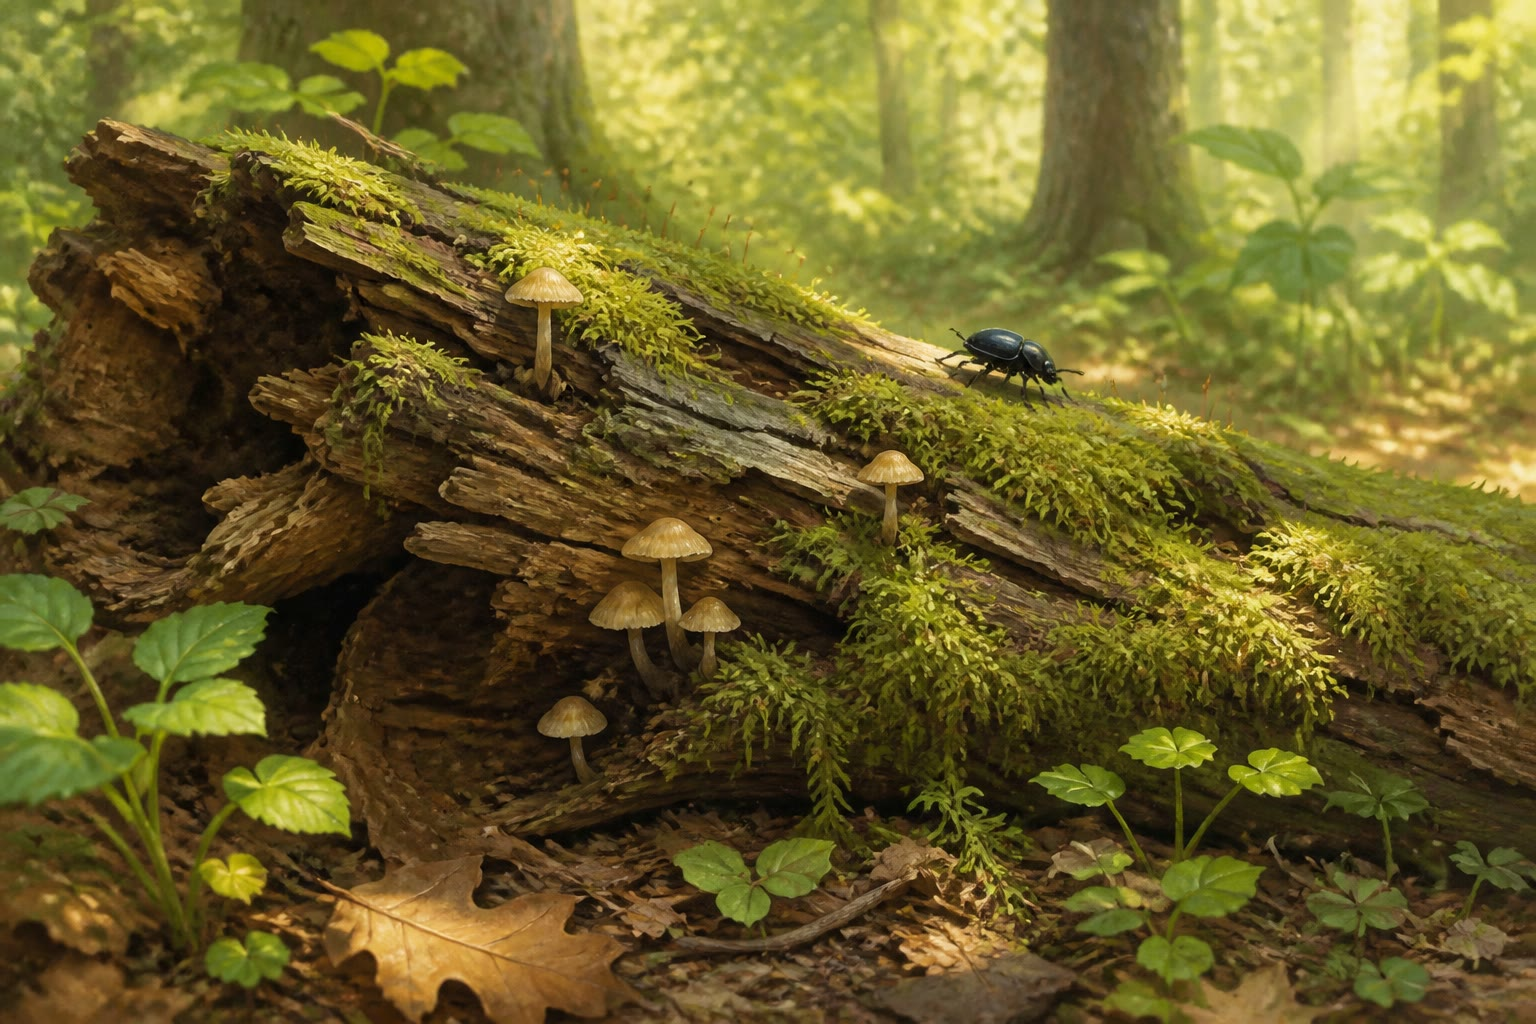
\includegraphics[width=0.62\linewidth]{images/book1/ai/g2-nature-log.jpg}

{\small 这根腐烂的原木其实是一座“宫殿”：顶上长着苔藓，
墙上长着蘑菇，走廊里有一只甲虫。}
\end{omfigure}

\begin{remark}[我们也是其中一员]\label{rem:g2:caring-for-nature:part}
人也是\omterm{def:g1:living-or-not:living}{生物}：我们呼吸的空气、喝的水和吃的食物，
都来自\omterm{def:g2:caring-for-nature:environment}{自然}。照顾\omterm{def:g2:caring-for-nature:environment}{自然}，
不只是对兔子的善意，也是在照顾我们自己赖以生存的世界，
正如\cref{ch:g2:where-animals-live}中所说，
每一个\omterm{def:g2:where-animals-live:habitat}{栖息地}都是如此。
\end{remark}

\section{什么有害，什么有益}

\begin{proposition}[小行动，真伤害]\label{prop:g2:caring-for-nature:harm}
在\omterm{def:g2:caring-for-nature:environment}{自然}中，伤害很少出于想做坏事，
而是源于没有多想：
\begin{itemize}
  \item 乱扔的垃圾会留存多年，可能困住或毒害\omterm{def:g1:animals-around-us:animal}{动物}；
  \item 把花全部摘光，就没有花能结\omterm{def:g2:from-seed-to-plant:seed}{种子}了，
        也就没有花可供蜜蜂采蜜；
  \item 大声喧哗、追赶\omterm{def:g1:animals-around-us:animal}{动物}，
        会把它们从食物和幼体身边吓走；
  \item 踩坏河岸、翻乱石头、折断树枝，
        都会毁掉一个小小的家。
\end{itemize}
\end{proposition}
\admitted

\begin{example}[瓶盖]\label{ex:g2:caring-for-nature:cap}
一个随手丢下的塑料瓶盖对我们来说不算什么，却会在草地上留存很多很多年——
久到大人都有了孩子，孩子还能找到同一个瓶盖。
自然界没有垃圾车：我们留下的东西，
都会留在那里。
\end{example}

\begin{method}[游客守则]\label{met:g2:caring-for-nature:rules}
在野外时：
\begin{enumerate}
  \item 把所有垃圾都带回家，一样也不留；
  \item 观赏\omterm{def:g1:plants-around-us:parts}{花朵}、昆虫和鸟巢，而不是采集它们；
        只摘极少数常见的花，
        绝不把一丛花全部摘光；
  \item 翻开的每一块石头和每一段原木都要放回原处，
        下面可能住着\omterm{def:g1:living-or-not:living}{生物}；
  \item 在靠近河岸等脆弱地点时，沿小路行走；
  \item 远远地、安静地观察\omterm{def:g1:animals-around-us:animal}{动物}，
        不要打扰它们的幼体。
\end{enumerate}
离开时，要让别人看不出你曾经来过。
\end{method}

\begin{example}[主动去帮忙]\label{ex:g2:caring-for-nature:help}
照顾还可以超越“不伤害”。热浪中放一碟水，
花园里留一小块不割草的野生角落，冷天里为鸟类撒些\omterm{def:g2:from-seed-to-plant:seed}{种子}，
以及像
\cref{ex:g2:where-animals-live:schoolpond}那样的校园池塘：
每一样都能为一些\omterm{def:g1:living-or-not:living}{生物}提供食物、水，或是它们失去的家。
\end{example}

\section{分类与节约}

\begin{proposition}[废物可以再利用]\label{prop:g2:caring-for-nature:recycle}
我们丢掉的很多东西都可以再次使用。
对废物进行\emph{分类}\index{废物分类}——玻璃归玻璃，纸归纸，果皮归堆肥——
这样玻璃瓶能变成新的玻璃瓶，
果皮能变成土壤，而不是全都堆积起来。
而被\emph{节约}的东西——水、纸张、电——
根本不会变成废物。
\end{proposition}
\admitted

\begin{example}[堆肥桶]\label{ex:g2:caring-for-nature:compost}
苹果核和胡萝卜皮放进堆肥桶里，会慢慢变成深色、松散的土壤，
这离不开蚯蚓、鼠妇以及肉眼看不见的微小\omterm{def:g1:living-or-not:living}{生物}的帮助。
到了明年春季，这些土壤能为番茄提供养分。
什么都没有被浪费，果皮
重新回到了生命的循环之中。
\end{example}

\begin{remark}[小手也能帮忙]\label{rem:g2:caring-for-nature:count}
刷牙时关掉水龙头，纸张两面都用，
用堆肥桶，把垃圾带回家：每一件都很小，
但有上百万人在做——或者不做。\omterm{def:g2:caring-for-nature:environment}{自然}是否被照顾或伤害，
主要取决于像你这样日常的小小选择。
\end{remark}

\section{练习}

\begin{exercise}[$\star$]\label{exo:g2:caring-for-nature:1}
什么是\omterm{def:g1:living-or-not:living}{生物}的\omterm{def:g2:caring-for-nature:environment}{环境}？
说出你身边三样来自\omterm{def:g2:caring-for-nature:environment}{自然}的东西。
\end{exercise}

\begin{exercise}[$\star$]\label{exo:g2:caring-for-nature:2}
当腐烂的木头被踢散时，谁会失去家园？
从\cref{ex:g2:caring-for-nature:home}中说出三种居住者。
\end{exercise}

\begin{exercise}[$\star$]\label{exo:g2:caring-for-nature:3}
给出\cref{met:g2:caring-for-nature:rules}中的四条游客规则。
\end{exercise}

\begin{exercise}[$\star$]\label{exo:g2:caring-for-nature:4}
为什么垃圾必须由我们带回家？
请用\cref{ex:g2:caring-for-nature:cap}中的瓶盖来回答。
\end{exercise}

\begin{exercise}[$\star$]\label{exo:g2:caring-for-nature:5}
为什么我们不应该摘走一丛花中的所有\omterm{def:g1:plants-around-us:parts}{花朵}？
给出\cref{prop:g2:caring-for-nature:harm}中的两个理由。
\end{exercise}

\begin{exercise}[$\star$]\label{exo:g2:caring-for-nature:6}
苹果核在堆肥桶里会发生什么变化？
谁来完成这项工作，我们最后得到什么？
\end{exercise}

\begin{exercise}[$\star$]\label{exo:g2:caring-for-nature:7}
从\cref{ex:g2:caring-for-nature:help}中，
给出两种有意帮助\omterm{def:g2:caring-for-nature:environment}{自然}的做法。
\end{exercise}

\begin{exercise}[$\star$]\label{exo:g2:caring-for-nature:8}
试一试：下次散步时，数一数你看到多少件垃圾
（不要碰危险的物品），哪一种最多？
每一种原本应该放到哪里？
\end{exercise}

\begin{exercise}[$\star\star$]\label{exo:g2:caring-for-nature:9}
在池塘边，艾玛想把三只\omterm{ex:g2:animals-grow-up:frog}{蝌蚪}装进罐子里带回家，
“好让它们安全地长大”。请结合本章和
\cref{exo:g2:where-animals-live:10}，你会建议她
改为怎样做？
\end{exercise}

\begin{exercise}[$\star\star$]\label{exo:g2:caring-for-nature:10}
“一个瓶盖算不了什么。”请利用
\cref{rem:g2:caring-for-nature:count}来回答：会发生什么？
如果一百万名游客都想着同一句话——朝坏的方向想，
也朝好的方向想？
\end{exercise}
